\documentclass{mcmthesis}
\renewcommand{\headset}{{2019}\\MCM\\Summary Sheet}
\mcmsetup{CTeX = true,tcn = 1234,problem = A,sheet = true, titleinsheet = true, keywordsinsheet = true,titlepage = false, abstract = true}
\iffalse
\bibliography{reference.bib}
\fi
\usepackage{indentfirst}
\setlength{\parindent}{2em}
\usepackage{palatino}
\usepackage{lipsum}
\usepackage{booktabs} %三线表
% \usepackage{parskip} %禁止首行缩进{}
% \setlength{\parindent}{0cm} %禁止首行缩进
\usepackage{graphicx} %插入图形
\usepackage{makecell}
\usepackage{cite}
\bibliographystyle{unsrt}

\title{How to raise dragon scientifically}
\author{YeLingfeng  ZhangWeimin  Chengliye}
\date{\today}
\begin{document}
\begin{abstract}
\hspace{2em} How much does a dragon eat and how much space does a dragon need?
These questions may not be of interest to Daenerys alone. We all want to know the answers.
In this paper, we make some reasonable assumptions about the characteristics of dragons, 
such as diet, range, etc., and establish a hybird model for the growth process of dragons, 
and analyze the growth curve of dragons, energy requirements and its interraction with environment.

First, a growth model of dragon is established by analogy with the growth model of pig.
We found that the growth curve of the dragon was S-shaped, and its maximum weight could reach 200 tons. 
It could grow to 100 tons by the time it was around 210 years old.
On the basis of this simplified model, the amount of food a dragon needs to eat in order to gain weight is only related to the dragon's weight, 
with a 100 ton dragon probably consuming 1,678.25 kilograms of food for every 1 kilogram gained.

Secondly, we analyze the daily energy intake and expenditures of the dragon.
We calculated the weight of meat that a dragon needs to eat to maintain its life activity and weight. An adult dragon need $903.76kg$ fresh meat to eat. The relationship between energy that dragon consume and his weight is deducted.

Then we constructed a dragon habitat, which changes dynamically according to the range of activity of the dragon and the activity of its prey.
To the simplicity of calculation, we divide the nutritional structure of ecosystem into two categories: plants and animals. Dragons eat animals only. And the area of the habitat is calculated when it can support an adult dragons. It is calculated that at least 15,000 square kilometers of temperate grassland ecosystem are needed to support the normal growth of an adult dragon that weights 100tons.

Finally, the influence of the activities of dragons to different ecosystem is discussed. Four ecosystem is considered. Grassland ecosystem and rainforest ecosystem can keep balance.
While the ice fields ecosystem and desert ecosystem may be seriously damaged eventually, and the dragons will fly away for lack of food.

\begin{keywords}
Energy Intake and Expenditures ; growth curve ; Impact on Ecosystem ;
\end{keywords}
\end{abstract}
\maketitle

\tableofcontents % 目录
\newpage


\section{Introduction}
~\ \
\subsection{Problem Background}
~\ \

A dragon is a large, serpentine legendary creature that appears in the folklore of many cultures around the world. 
The popular western image of a dragon is based on a conflation of earlier dragons from different traditions, 
and of inaccurate scribal drawings of snakes. 
In western cultures, dragons are portrayed as monsters to be tamed or overcome, usually by saints or culture heroes, 
as in the popular legend of Saint George and the Dragon. 
They are often said to have ravenous appetites and to live in caves, where they hoard treasure. 
These dragons appear frequently in western fantasy literature, including The Hobbit by J. R. R. Tolkien, 
the Harry Potter series by J. K. Rowling, and A Song of Ice and Fire by George R. R. Martin.

The dragons we will talk about here are the three dragons raised by Daenerys Targaryen, the "Mother of Dragons".
When hatched, the dragons are small, roughly 10 kg, and after a year grow to roughly 30-40 kg. 
They are able to fly great distances, breath fire, and resist tremendous trauma.

~\ \
\subsection{Restatement of the Problem}
~\ \

Consider the three dragons in The Song of Ice and Fire are living today. We want to help Daenerys get to know how to raise them.
The major problems are discussed in this paper, which are:

\begin{itemize}
    \item What are the dragon's characteristics?
    \item What is the relationship between the weight and age of a dragon?
    \item How much do dragon eat to sustain life?
    \item How large is the habitat to support three dragons?
    \item How do the dragons interact with their environment?
\end{itemize}

~\ \
\subsection{Our Work}
~\ \

In order to solve these problems, our jobs as follow:

\begin{enumerate}[\bfseries 1.]
    \item Build a model to pridict the growth process of dragon.
    \item Calculate the critical energy intake of dragon to maintain life.
    \item Build a simple ecosystem with only three trophic levels and simulate the activity of dragons
    \item Analyse dragons' impact on ecosystem.
\end{enumerate}

~\ \
\section{Assumptions}
~\ \

To make the model's predictions more accurate, 
we made some assumptions about the characteristics and behavior of dragons as follow:

\begin{itemize}
    \item Dragons have a long life span.
    \item It's difficult for dragons to breed.We just think about the three dragons all along.
    \item Dragons can fly long distances, but they don't need to fly long distances to prey.
    \item The dragon only eats meat, which means it is at least a third trophic level. And their favourate food is lamb, as the book says.
    \item The growth curve of dragons has a sigmoid form.
    \item Dragons have been growing up all their lives, but it is not sure how long they can live and how big they are. It is believed that the size of dragons is limited by their growing environment, and the older the dragons are, the larger they are.
\end{itemize}

~\ \
\section{The Growth Model of Dragon}
~\ \

There are recognised difficulties in applying mathematical methods
to model development in animals. Living organisms entail not only the
notion of biological function or purpose but also the notion of growth and
development that differentiates biology from other natural sciences.

The two most classical modelling techniques of biological
phenomena are continuous-time, and discrete-time models. A number of
biological objects do not fit either form; such systems contain
heterogeneity, where some phenomena are continuous while some are
discrete.The modelling of this kind of systems would then naturally involve
two different parts, a continuous one in ordinary differential equations, and a
discrete one in difference equations, yielding what is called a ‘hybrid’ system. 

We use V.L.Stass's research on the prediction of the growth of pigs for reference, 
and make some improvement on the model for the prediction of the growth of dragons.
It should be noted that in this model, food is infinite.

The symbols used in this model are listed in Table \ref{tb:Variables1}.

\begin{table}[h]
\centering
\caption{Symbols in Growth Model}
\begin{tabular}{cll}
\toprule
\textbf{Symbols}   & \textbf{Description}                                        &\textbf{Unit}    \\
\midrule
$M$                & Current weight of dragon                                    &kg               \\
$m$                & Initial weight                                              &kg               \\
$m_{0}$            & Weight of dragon when one year old                          &kg               \\
$t$                & Current time, measured from birth                           &year             \\
$t_{0}$            & One year old                                                &year             \\
$K$                & A Intermediate variable, nondimensional                     &                 \\
$Z$                & current feed conversion coefficient                         &                 \\
\bottomrule
\end{tabular}\label{tb:Variables1}
\end{table}
explanation:
\begin{itemize}
\item $m_{0}=40$
\item $t_{0}=1$
\item $Z=n$ means that a dragon needs $nKg$ Pig feed to gain $1Kg$, while one kilogram of pig feed contains $17MJ$ of energy.
\end{itemize}

Bellerion, the oldest and largest dragon in the tangurian family, lived for 200 years and was so big that he could swallow an entire mammoth in one gulp.
We estimate that his weight is 100 tons.So $M_{x}=100000$ is considered as the minimum value of the maximum value of $M$.

In V.L.Stass’s model, the parameter '$K$' has been defined as the following form:
\begin{equation}
    K=\frac{M\cdot t}{m_{0}(2t-t_{0})}
\end{equation}

And we have following relationship between $K$ and $Z$:
\begin{equation}
    \frac{t-Kt_{0}}{t}=-\frac{(8K-Z)\cdot (K-1)}{4ZK}
\end{equation}

Substituting (2) into (1) and after obvious transformations, one get
\begin{equation}
    Z=8\cdot \frac{1-K}{\frac{M}{m_{0}}-2K+\frac{1}{K}}
\end{equation}

At this stage, it is necessary to calculate $Z_{x}$ to derive relevant relationships. 
As the first step, it is shown how to find parameter $'K'$ under the condition $M = M_{x} = 100000 kg$. 
In formal notation: $K|(M=M_{x}) = K_{x}$. We assume that (4) converges as $M\rightarrow M_{x}$,
and the following limit holds:
\begin{equation}
    \lim_{M \to M_{x}}(\frac{24.55K-1}{K+1})=\sqrt{24.55^{2}-1}, where (K\rightarrow K_{x}|_{M\rightarrow M_{x}})   
\end{equation}
It follows from (4) that under condition ($K= K_{x}$), $K_{x} = 1252.98$.

The next step is to calculate $Z_{x}$, $Z|(M=M_{x})(K=K_{x}) = Z_{x}$.

Substituting $K_{x}$ and $M_{x}$ into (3) one obtains $Z_{x}= 1678.25$. $Z_{x}$ an
analytical expression that will be presented in sections below. One should
notice that $Z_{x}$ and $K_{x}$ are constants both linked to $M_{x}=100000Kg$.
$Z$ has a clear biological interpretation.

From ($K_{x}=1252.98$)($M_{x}=100000$) follows that $t|(M=M_{x})(K=K_{x}) = t_{x} = 209.921$
years. This means that under the model conditions, dragons can reach $M_{x}$ in $209.921$ years, 
consuming $1678.25\cdot 17 MJ$ of feed to put on the last kilogram. 

There is a standard procedure of how to find the maximum $M_{x}$. The
condition that $M_{x}$  has maximum is $\frac{dM_{x}}{dK_{x}} = 0$. 
It follows $max Mx= Mxx = 4m_{0}K_{x} = 200476.8 kg.$

It is widespread opinion that the growth rate in many mammals has a sigmoid form (Li , Wu, 2010).
Here we assume that dragon has the same characteristic.

Now we have some data as follow:
\begin{itemize}
    \item When $t=0$, $M=10$.
    \item When $t=1$, $M=40$.
    \item When $t=209.921$, $M=100000$.
    \item When $t\rightarrow \infty $, $M\rightarrow 200476.8$.
\end{itemize}

From this we derive an expression for M with respect to T:
\begin{equation}
    M=\frac{d}{1+e^{-a(t-c)}}+b
\end{equation}
Among them
\begin{align*}
a&=2.43265339\times10^{-2} & b&=-1.21593407\times10^{3}\\
c&=2.09424176\times10^{2} & d&=2.01215934\times10^{5}
\end{align*}

The relation is shown in Figure \ref{Figure_1}
\begin{figure}[!htbp]
\centering
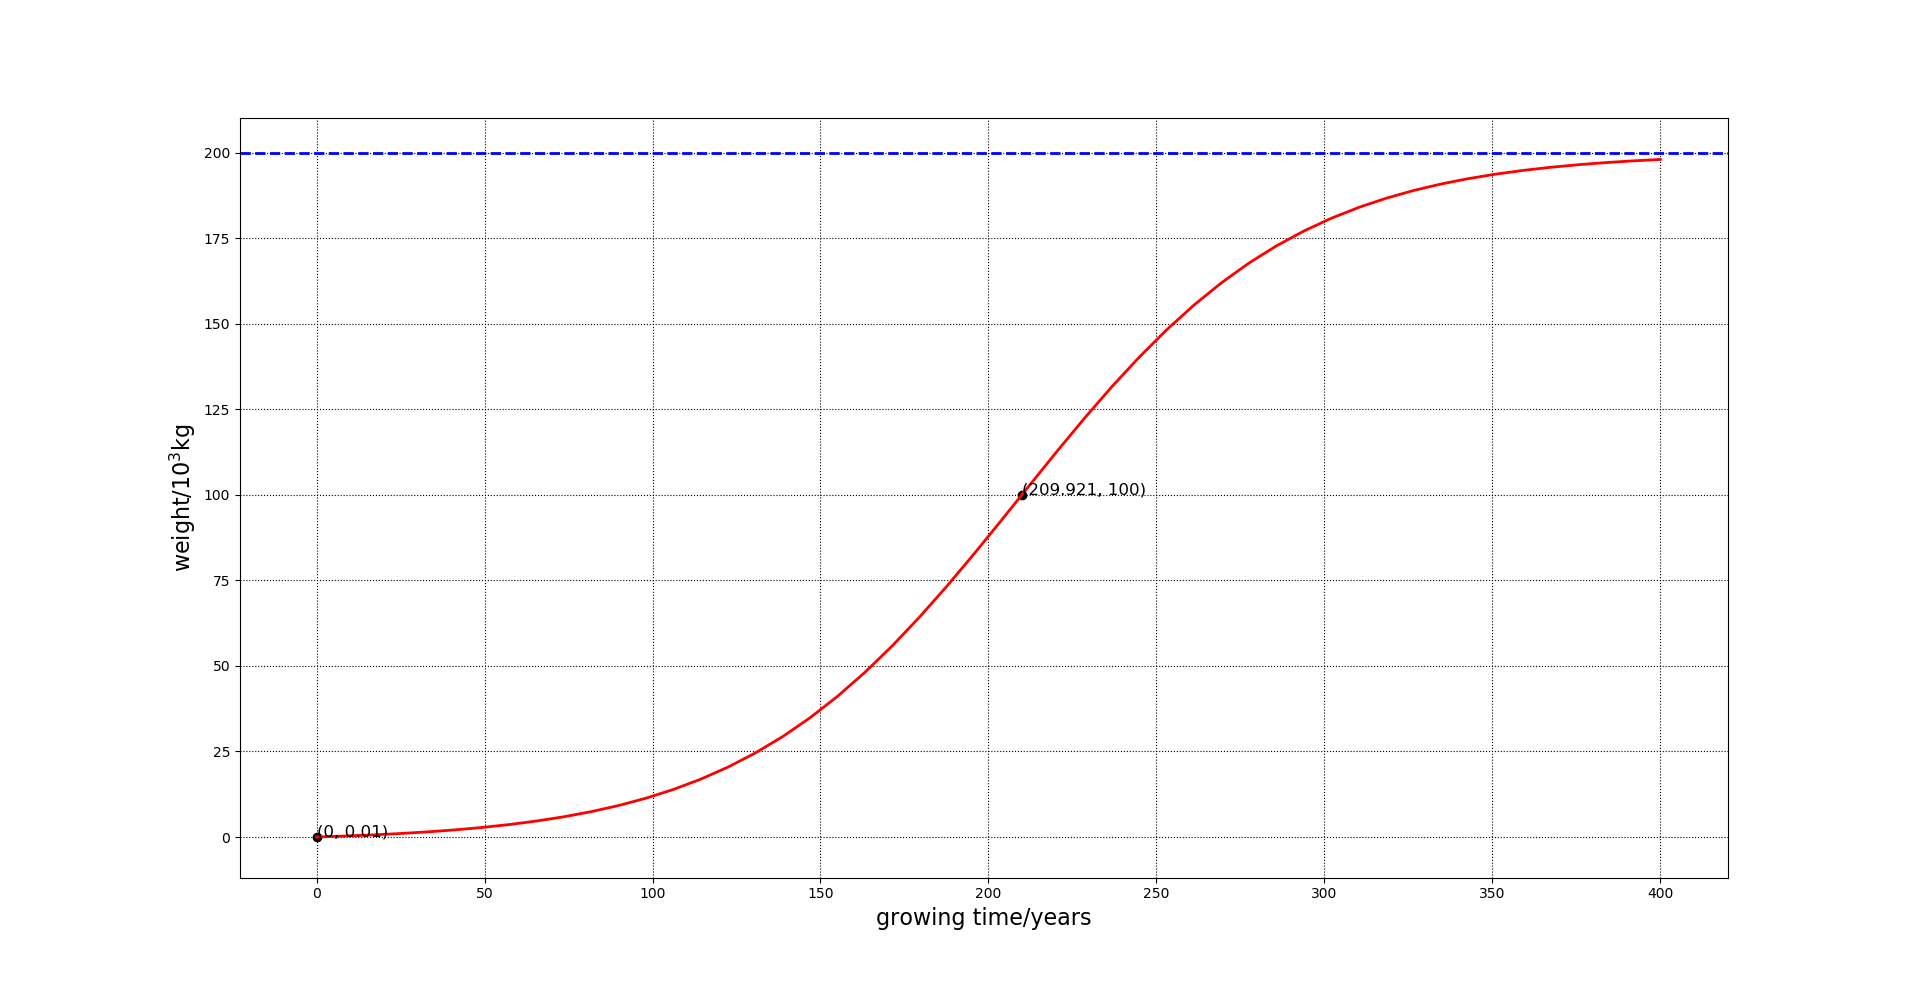
\includegraphics[width=40em]{Figure_1.png}
\caption{The relation of M and t}\label{Figure_1}
\end{figure}

~\ \
\section{The Model of Energy Intake}
~\ \

The symbols to be used in this chapter are shown in Table \ref{tb:Variables2}.
\begin{table}[h]
\centering
\caption{Symbols in Energy Intake Model}
\begin{tabular}{cll}
\toprule
\textbf{Symbols}   & \textbf{Description}                                &\textbf{Unit}   \\
\midrule
$R_{FM}$           & field metabolic rates                               &kJ/days             \\
$DMI$              & dry matter intake                                   &g                   \\
$FMI$              & fresh matter intake                                 &g                   \\
$M$                & weight                                              &g                   \\
$R_{F}$            & feeding rates                                       &(DMI)/d or (FMI)/d  \\
$E_{d}$            & the metabolisable energy content of animals' diet   &kJ/g                \\
$G$                & the food a dragon need to eat a day                 &g                   \\
\bottomrule
\end{tabular}\label{tb:Variables2}
\end{table}

One of the first questions people ask about a wild animal is “What does it eat?” To answer what does dragon eat 
and how much energy it get from food, we refer to Kenneth A. Nagy's data. Referring to feeding rates by 79 species of mammals, 95 species of birds and 55 species of reptiles  estimated from doubly labeled water- based measurements, we get the following model to measure the intake of a dragon.\\

Feeding rates mean intake of both dry matter and fresh matter. 
Feeding rates are those needed to provide the metabolizable energy the animals burn in the field, so they represent “steady-state” conditions.
The FMR for a species, in units of kJ/d, was divided by the metabolisable energy content of its diet, 
either in units of metabolisable kJ/g dry matter or in units of metabolisable kJ/g fresh matter, 
to calculate feeding rates in units of g dry matter intake (DMI)/d or in units of g fresh matter intake (FMI)/d.
\begin{equation}
R_{F} = \frac{R_{FM}}{E_{d}}
\end{equation}
After analyzing a large number of data, the author obtains this formula: $R_{F} $ (DMI/d) satisfy
\begin{equation}
R_{F} = 0.323 \cdot M^{0.744}
\end{equation}

Because DMI means dry matter intake, to calculate the weight of dragons' food, it should be devided by moisture content.
Dragons's prey includes carnivores and herbivores, so there are 68\% water for an omnivore’s diet which means dragons eat omnivores.
According to this paper, meat contains energy 1490 cal/pound on average. And it is easily transformed to 13.7965 kJ/g.
In conclusion, the food a dragon need to eat a day can be calculated as follows:
\begin{equation}
F = \frac{0.323 \cdot M^{0.744}}{1-68\%}\cdot13.7965
\end{equation}

And one $kJ$ can be transformed to 238.9 calorie. The energy a dragon need $238.9F$ have the relationship with his weight like above.
After substituting data into formulas above, an adult dragon that 100 tons needs to eat $916.299$ calories (3.83549$kJ$) a day.


~\ \
\section{The Model of Interaction with Environment}
~\ \

Through the two models above, the dragons' growth curve and energy intake has been ensured. In this chapter,
the interaction between dragons and the environment will be disgussed. 
we first built a simplified ecosystem model which only lives the first trophic level and the second trophic level, 
adjusted the parameters to reach equilibrium, and then put dragons as top consumers into the model to see 
if the new equilibrium could be reached, or if the dragons could never get enough food to grow and leave the ecosystem.

~\ \
\subsection{Environment without dragon}
~\ \

In the simplified ecosystem model, we only consider the interactions between plants and animals,
and the primary variables used in this model are listed in Table\ref{tb:Variables3}

%表格位置需调整
\begin{table}[h]
\centering
\caption{Symbols in Energy Intake Model}
\begin{tabular}{cl}
\toprule
\textbf{Symbols}   & \textbf{Description}                                 \\
\midrule
$F$                & Sum of plants                                        \\
$M_{F}$            & Maximun number of plants in the ecosystem            \\
$R_{F}$            & Daily growth of plants                               \\
$S$                & Sum of animals                                       \\
$H_{S}$            & Maximum number of animals that ecisystem can support \\
$R_{S}$            & Daily growth of animals                              \\
$E$                & Amount of plants animal consume each day             \\
\bottomrule
\end{tabular}\label{tb:Variables3}
\end{table}

Without loss of generality, we make the following assumptions:
\begin{enumerate}
    \item The number of original plants is $F_{0}=2000$
    \item The number of original animals is $S_{0}=30$
    \item $M_{F}=10000$
    \item $R_{F}=0.02$
    \item $S_{F}=0.007$
\end{enumerate}

And we have following relations:
\begin{equation}
    \frac{\varDelta S}{\varDelta t}=R_{S}\cdot S_{0}\cdot \frac{H_{S}-S_{0}}{H_{S}}
\end{equation}
\begin{equation}
    \frac{\varDelta F}{\varDelta t}=R_{F}\cdot (F_{0}-E)\cdot \frac{M_{F}-F_{0}}{M_{F}}-E
\end{equation}
\begin{equation}
    H_{S}=\frac{8F_{0}}{15}
\end{equation}

The above several formulas give the relationship between the quantity of animals and the quantity of plants over time.

Formula $(9)$ points out that the change in the quantity of animals is positively correlated with the quantity of the previous day, and is also related to the difference between the upper limit of the quantity of animals that can be accommodated in the ecosystem and the actual quantity of animals--when the actual quantity of animals does not reach the environmental capacity,it means that more animals can be accommodated. On the contrary, various conditions in the natural environment will limit and reduce the quantity of excess. A specific parameter is selected so that the above relationship can be expressed in the form of an equation.

Fomula $(10)$ shows how the quantity of plants changes over time. The increase in the quantity of plants in a certain period of time is obviously composed of two parts--the increase determined by its current quantity and the quantity consumed by factors such as animals. $R_F$ determines how fast a certain amount of plants can grow, $F_0-E$ indicates how much plants are "left" after begin consumed at the last time point. The meaning of the fraction is basically similar to that mentioned in Equation$9$. The environmental capacity will have a specific impact on its maximum quantity and growth rate.

Fomula $(11)$ gives a simple conclusion that the maximum quantity of animals are strictlly limted by the amount of plants.

It is important to note that, the number of plants and animals we discuss here, does not mean the actual quantity, but a generalization of the concept of measurement, for instance, F = 1 can be here on behalf of the ecological system have 2 kilograms of forage grass and 3 kg of apple trees, then the corresponding F = 2 on behalf of the ecological system with 4 kilograms of forage grass and 6 kg apple tree.

Let $\Delta t=1day$ ,and we get the curve of population change in figure\ref{Figure_2}:
\begin{figure}[!htbp]
\centering
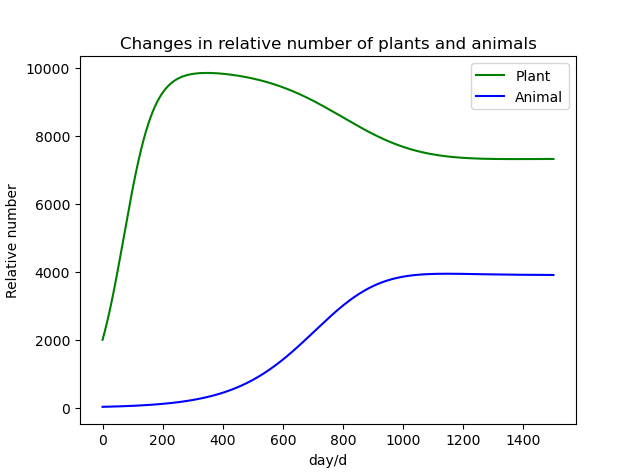
\includegraphics[width=30em]{Figure_2.png}
\caption{The relation of M and t}\label{Figure_2}
\end{figure}

We found that around $t=1200days$, the ecosystem region reaches stable, and the number of plants and animals at this time stabilizes at 7300 and 3900.In the following, we will add dragons to the ecosystem to explore the interaction between dragons and the environment.

~\ \
\subsection{Dragon's Interaction with Environment}
~\ \

On the basis of the above model, some additional assumptions are made in order to study the changes of the ecosystem after the putting dragons into the ecosystem.
\begin{enumerate}
    \item By the time dragons were put in, the ecosystem had reached equilibrium.
    \item We divided the entire ecosystem into rectangles of equal size, with each rectangle representing the maximum range the dragon could move in a day.
    \item Each day the dragon can eat only the animals in its rectangle.
    \item At the beginning of each day, the animals were evenly distributed throughout the area based on the distribution of plants.
    \item The dragon will always moves to the matrix with the most animals among its rectangle and the four adjacent rectangles every morning.
    \item If the dragon does not get enough food for five days in a row, it will leave.
\end{enumerate}

The variables we used in this model are listed in Table\ref{tb:Variables4}


\begin{table}[!htbp]
\centering
\caption{Symbols in Environment Model}
\begin{tabular}{cll}
\toprule
\textbf{Symbols}   & \textbf{Description}                                   \\
\midrule
$E$                & The number of animals a dragon needs to eat each day   \\
$F_{0}$            & The number of plants the day before                    \\
$R_{F}$            & Daily growth of plants                                 \\
$F$                & The updated number of plants                           \\
$S_{0}$            & The number of animals the day before                   \\
$S$                & The update number of animals                           \\
$M_{F}$            & Maximun number of plants in the ecosystem              \\
$H_{S}$            & Maximum number of animals that ecisystem can support   \\
$R_{S}$            & Daily growth of animals                                \\
\bottomrule
\end{tabular}\label{tb:Variables4}
\end{table}

We follow the following process for simulation:
\begin{enumerate}
    \item Calculate the number of plants and animals today by the total number of plants and the total number of animals from the previous day.
    \begin{equation}
        S=(1+R_{S}\cdot (H_{S}-S_{0})/H_{S})\cdot S_{0}
    \end{equation}
    \begin{equation}
        F=(1+R_{F}\cdot (M_{F}-F_{0})/M_{S})\cdot (F_{0}-E)
    \end{equation}
    \item Distributed animals evenly by the distribution of plants.
    \item Dragon moves to the matrix with the most animals.
    \item Calculate the amount of food the dragon needs to eat.
    \item Count up the plants and animals left.
\end{enumerate}

The initial distribution of plants is randomly generated, as shown in figure\ref{fig:simulate2}
\begin{figure}[h]
    \centering
    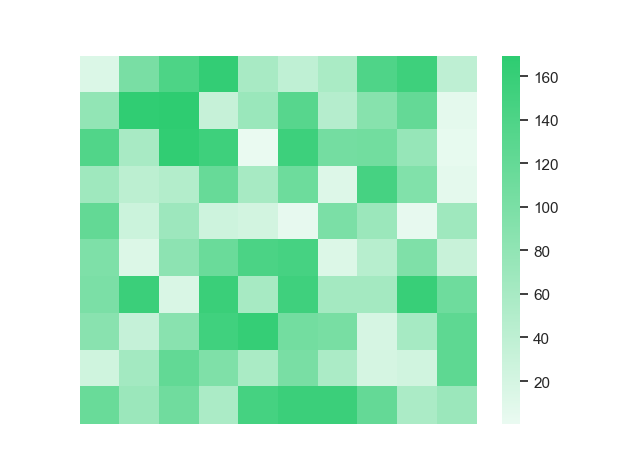
\includegraphics[width=25em]{Figure_3.png}
    \caption{An example of initialization of plants}\label{fig:simulate2}
\end{figure}

We found that when $L = 10$ and $E = 34$, the ecosystem will reach equilibrium, as shown in figure\ref{fig:simulate3} . While when $E = 35$, the dragon will leave after it enters, as shown in figure\ref{fig:simulate4} . When $E < 34$, the ecosystem will also reach equilibrium, but the amount of animals will reach a higher level, as shown in figure \ref{fig:simulate5}.\\

\begin{figure}[h]
    \centering
    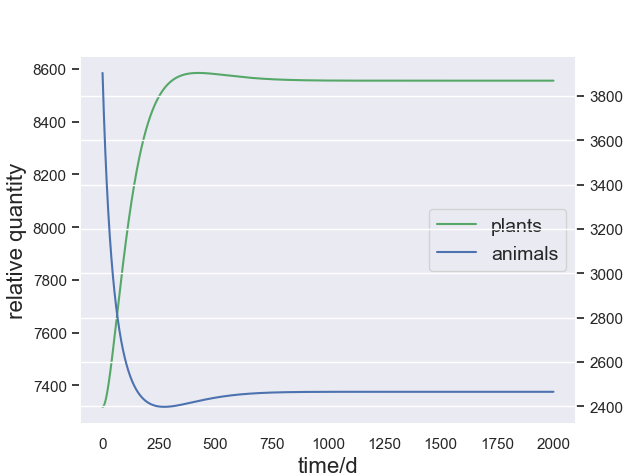
\includegraphics[width=25em]{Figure_4.png}
    \caption{Simulation image of $E=32$}\label{fig:simulate3}
\end{figure}
\begin{figure}[t]
    \centering
    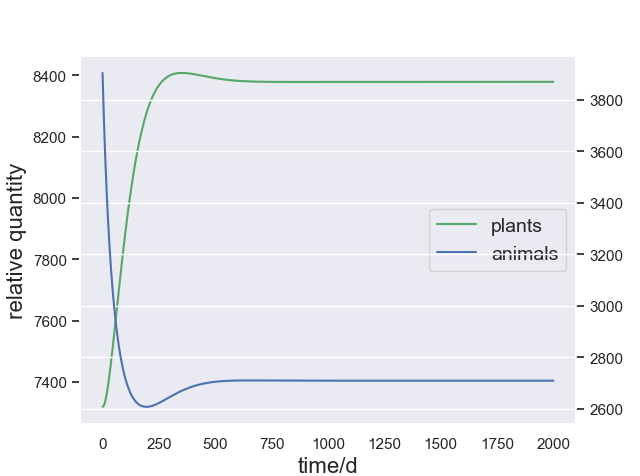
\includegraphics[width=25em]{Figure_5.png}
    \caption{Simulation image of $E=34$}\label{fig:simulate4}
\end{figure}
\begin{figure}[t]
    \centering
    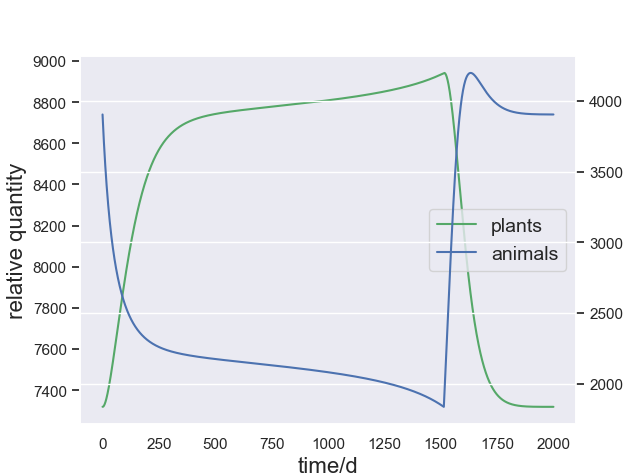
\includegraphics[width=25em]{Figure_6.png}
    \caption{Simulation image of $E=35$}\label{fig:simulate5}
\end{figure}
The images also show that when dragons were first put into the ecosystem, the animal population declined rapidly. If $E<34$, then the ecosystem will reach equilibrium in 300 days approximately. Otherwise, the number of animals would continue to decline until the dragons left after about 1500 days, and then equalized again after about 400 days.

We finally chose $E=34$ to describe the daily food requirement of the dragon, and we will give concrete arguments to explain the rationality of this choice in the following paragraphs.


~\ \
\subsection{The optimum environment and climate to support the growth of dragons}
~\ \

We have already discussed the growth curve of dragons(Chapter 3), the amount of energy required per day for a dragon of a given weight(Formula 8), and the requirements for maintaining balance in an ecosystem. And now we're going  to figure out what kind of environment would be suitable for dragons to grow under these conditions.

We use a energy transfer model to establish the relationship between energy consumption and the environment, the variables we used in this model are listed in Table\ref{tb:Variables5}


\begin{table}[h]
\centering
\caption{Symbols in Environment Model}
\begin{tabular}{cl}
\toprule
\textbf{Symbols}   & \textbf{Description}                                         \\
\midrule
$G_{R}$            & Ground radiation                                             \\
$\rho$             & Utility rate of luminous energy                             \\
$S$                & The scope of the dragon's daily activities,                  \\
$K$                & Energy transfer efficiency between different trophic levels  \\
$E_{0}$            & The Energy a 100-tons dragon needs every day                 \\
$S_{0}$            & The specific energy for $S=1$                                \\
\bottomrule
\end{tabular}\label{tb:Variables5}
\end{table}
Explanation:
\begin{itemize}
\item $\rho$ range from $0.5\%$ to $2\%$
\item $K$ we assume $S=150Km^{2}$
\item $E_{0}$ range from $10\%$ to $20\%$
\end{itemize}

From (8), we can figure out that
\begin{equation}
    E_{0}=3.83549\cdot 10^{8}kJ
\end{equation}

From the privious model, we have
\begin{equation}
    E_{0}=34\cdot S_{0}
\end{equation}

Then
\begin{equation}
    S_{0}=1.12808\cdot 10^{7}kJ
\end{equation}

In order to achieve ecological balance, we have the following equation:
\begin{equation}
    E_{0}=\frac{2}{3}\cdot \frac{S\cdot G_{R}\cdot \rho}{365}\cdot K^{2}
\end{equation}

Let $\rho=1\%$, we can figure out that
\begin{equation}
    G_{R}\approx 5.5998\cdot 10^{9} J/year
\end{equation}

This corresponds exactly to the ground radiation of the grassland ecosystem in the temperate zone (approximately $5\cdot 10^{9} J/year$)

\begin{figure}[!htbp]
    \centering
    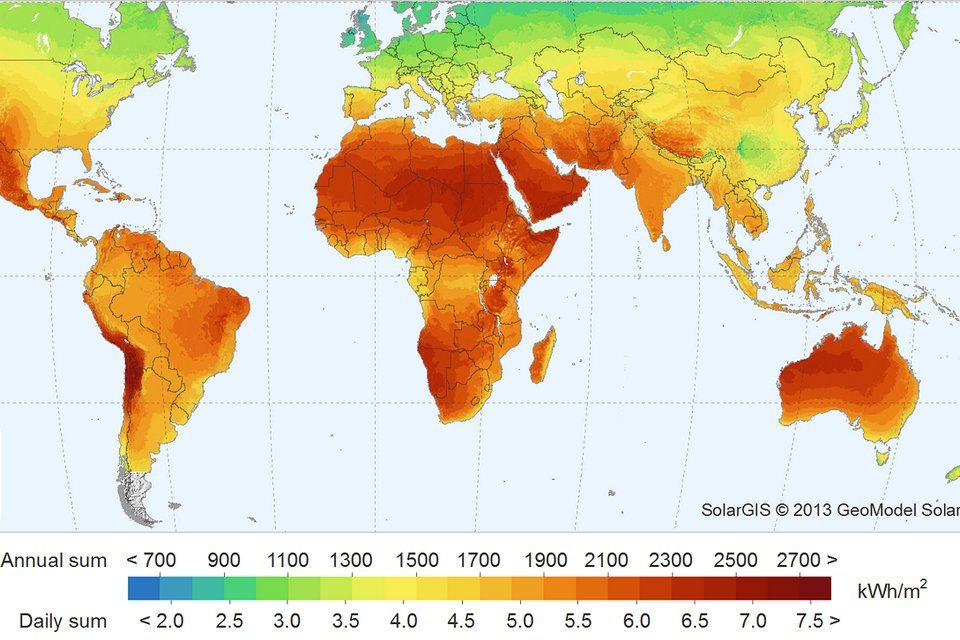
\includegraphics[width=30em]{Solar_radiation.png}
    \caption{Ground Radiation}
\end{figure}

At the same time, we can calculate $S_{0}$ again under this condition by the following equation:
\begin{equation}
    \frac{2}{3}\cdot \frac{S\cdot G_{R}\cdot \rho}{365}\cdot K = 24 \cdot S_{0}
\end{equation}

Figure out that $S_{0}=2.0845\cdot 10^{7}kJ$.
Though there is a certain deviation between this result and our previous results, they are on the same order of magnitude, so the error could be accepted.
This also validates the reasonability of taking $E=34$

Therefore, we can draw the following conclusion:

At least 15,000 square kilometers of temperate grassland ecosystem are needed to support the normal growth of an adult dragon that weights 100tons.


~\ \
\subsection{Interaction with Different Environments}
~\ \

The grassland ecosystem in the temperate zone has been proved to be an ideal living environment for adult dragons. It can maintain the balance of daily food intake and consumption of various life activities in this ecological environment. The grassland can also maintain the stability of the ecosystem in an appropriate area without collapse. What about other types of ecosystems? We selected several typical climate environments for discussion. They are: rainforest in the tropics, ice fields in the sub-frigid zone, and large deserts near the tropics.

It is not easy to estimate the energy that producers can fix in these types of ecosystems and perform the next calculation. Therefore, we have to make the following assumptions and estimates for the energy inflow of the ecosystem, that is, use the solar radiation per unit area to estimate. The relevant data is shown in the following table:
\begin{table}[h]
\centering
\caption{Symbols in Environment Model}
\begin{tabular}{cc}
\toprule
\textbf{Ecosystem Types}          & \textbf{Solar Radiation(Unit:$\frac{10^{8}J}{m^{2}\cdot year}$)}    \\
\midrule
rainforest in the tropics         &  70            \\
ice fields in the sub-frigid zone &  27            \\
deserts near the tropics          &  80            \\

\bottomrule
\end{tabular}\label{tb:Variables6}
\end{table}


After getting the amount of solar radiation, we estimate the inflow rate of ecosystem energy based on the ability of plants to fix solar energy. It should be noted that desert areas are not suitable for general efficiency, because the lack of water makes their vegetation coverage far unable to compare with grasslands or rain forests; similarly, appropriate adjustments are needed in the estimation of ice sheets, The cold temperature makes the survival of many creatures especially difficult.

After obtaining the energy obtained by the plant, we can correspondingly convert it into the "plant quantity" unit used in the previous section. By adjusting the parameters of the plant growth process, we can make it reach the new general animal and plant quantity where the balance is based on the fact that the number of plants in the balance is proportional to the number of fixed solar energy. As shown as follows, in the three ecological environments, the number of plants is finally fixed to 10220, 1048, 2309, and the corresponding animals The quantity is 5452, 559, 1230.

\begin{figure}[h]
    \centering
    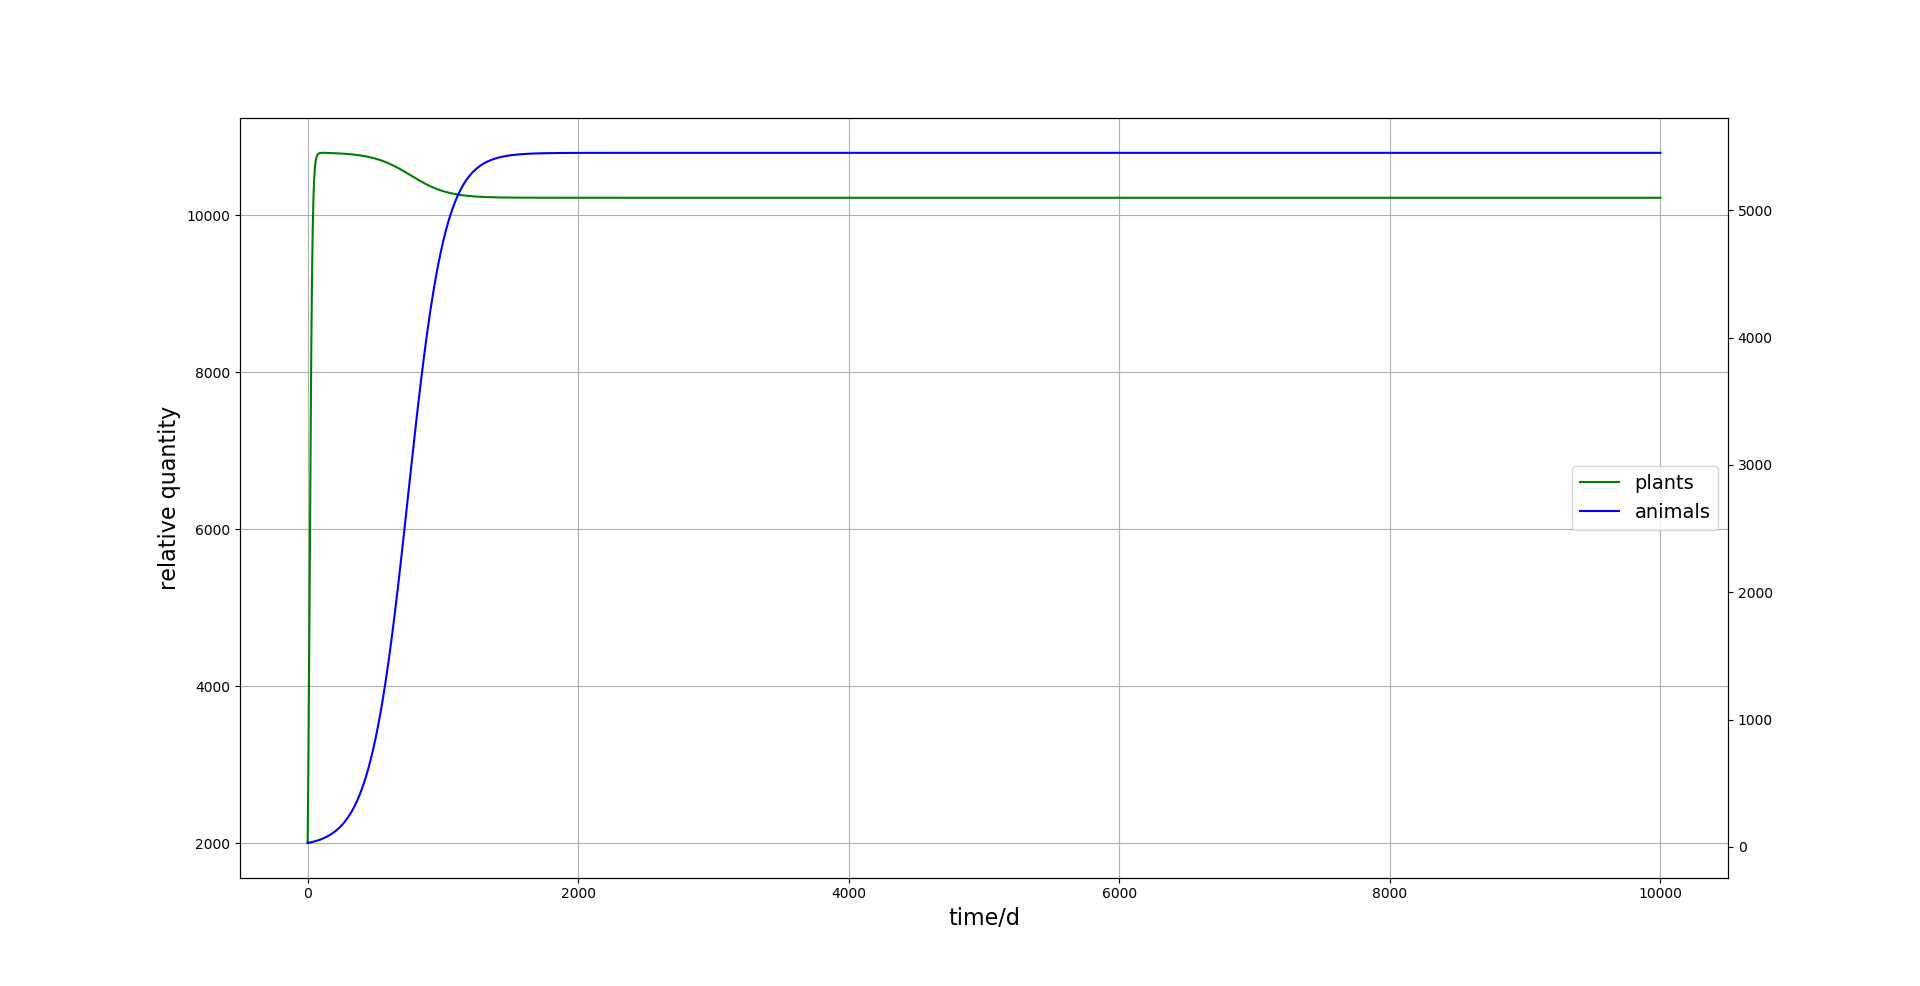
\includegraphics[width=35em]{Figure_7.png}
    \caption{rainforest}\label{fig:simulate6}
\end{figure}

\begin{figure}[h]
    \centering
    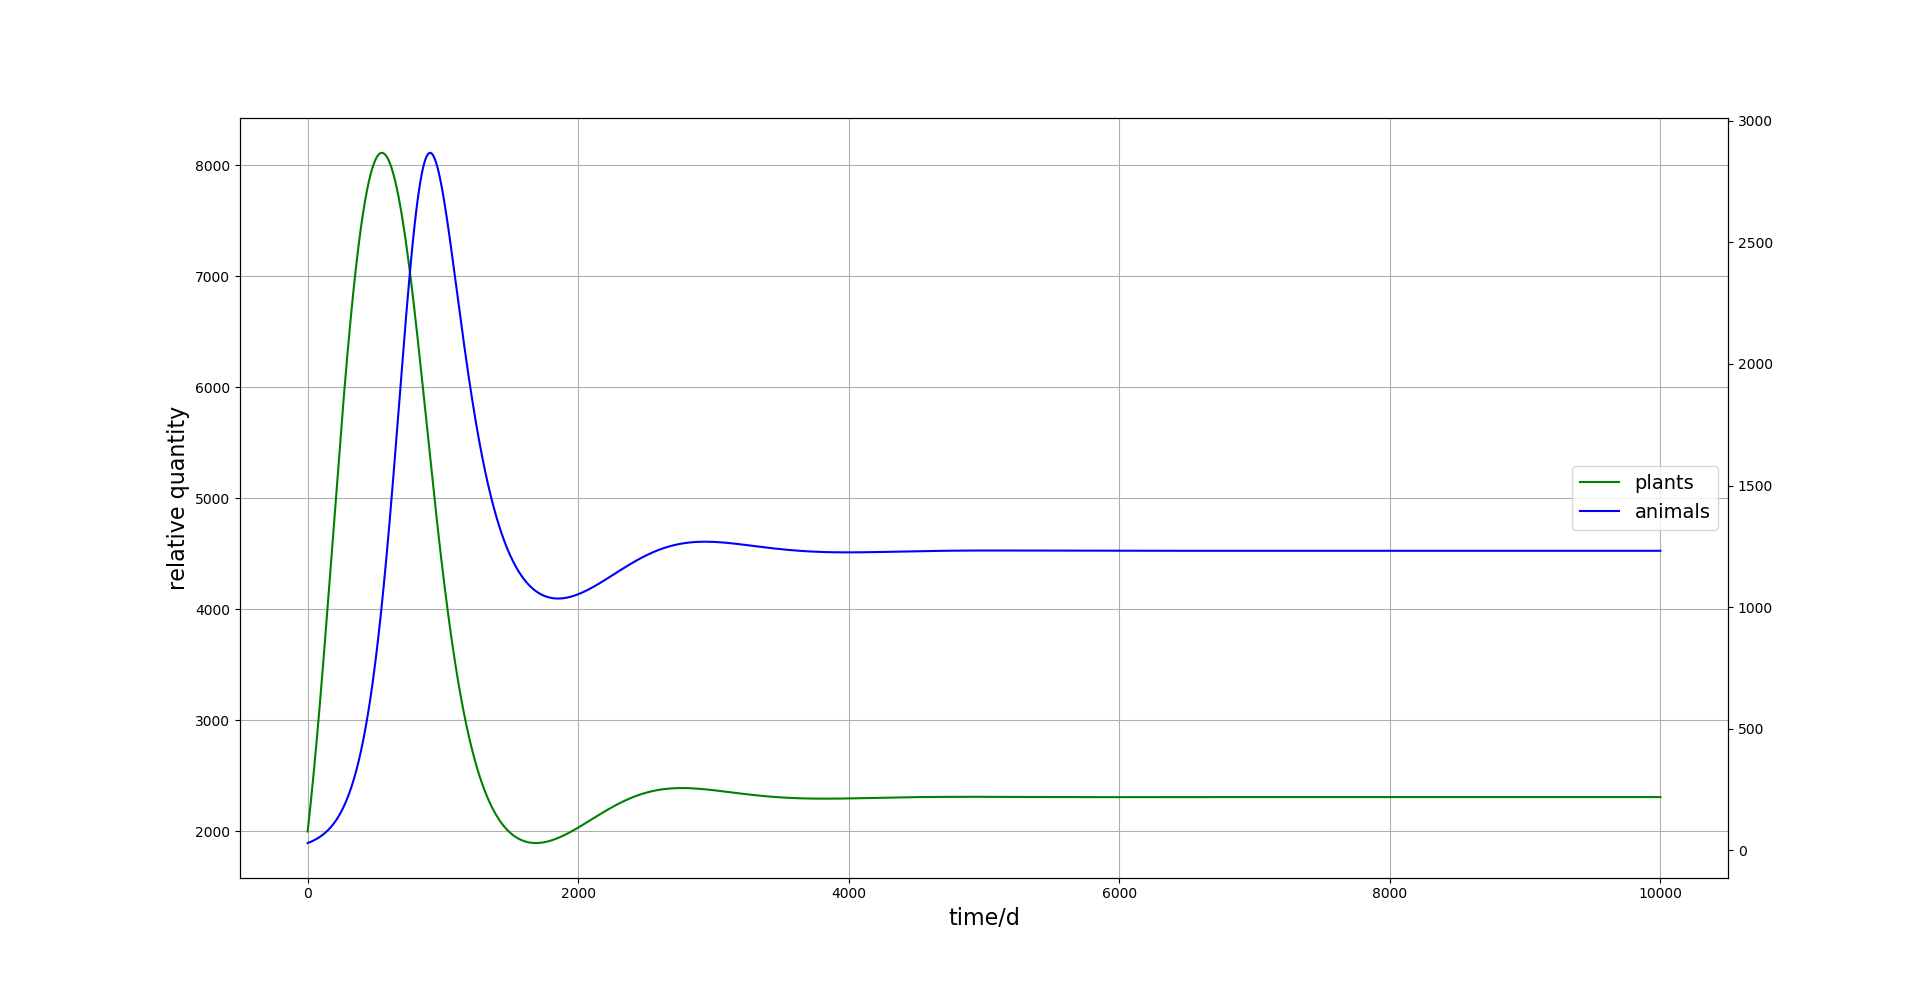
\includegraphics[width=35em]{Figure_8.png}
    \caption{ice fields}\label{fig:simulate7}
\end{figure}

\begin{figure}[h]
    \centering
    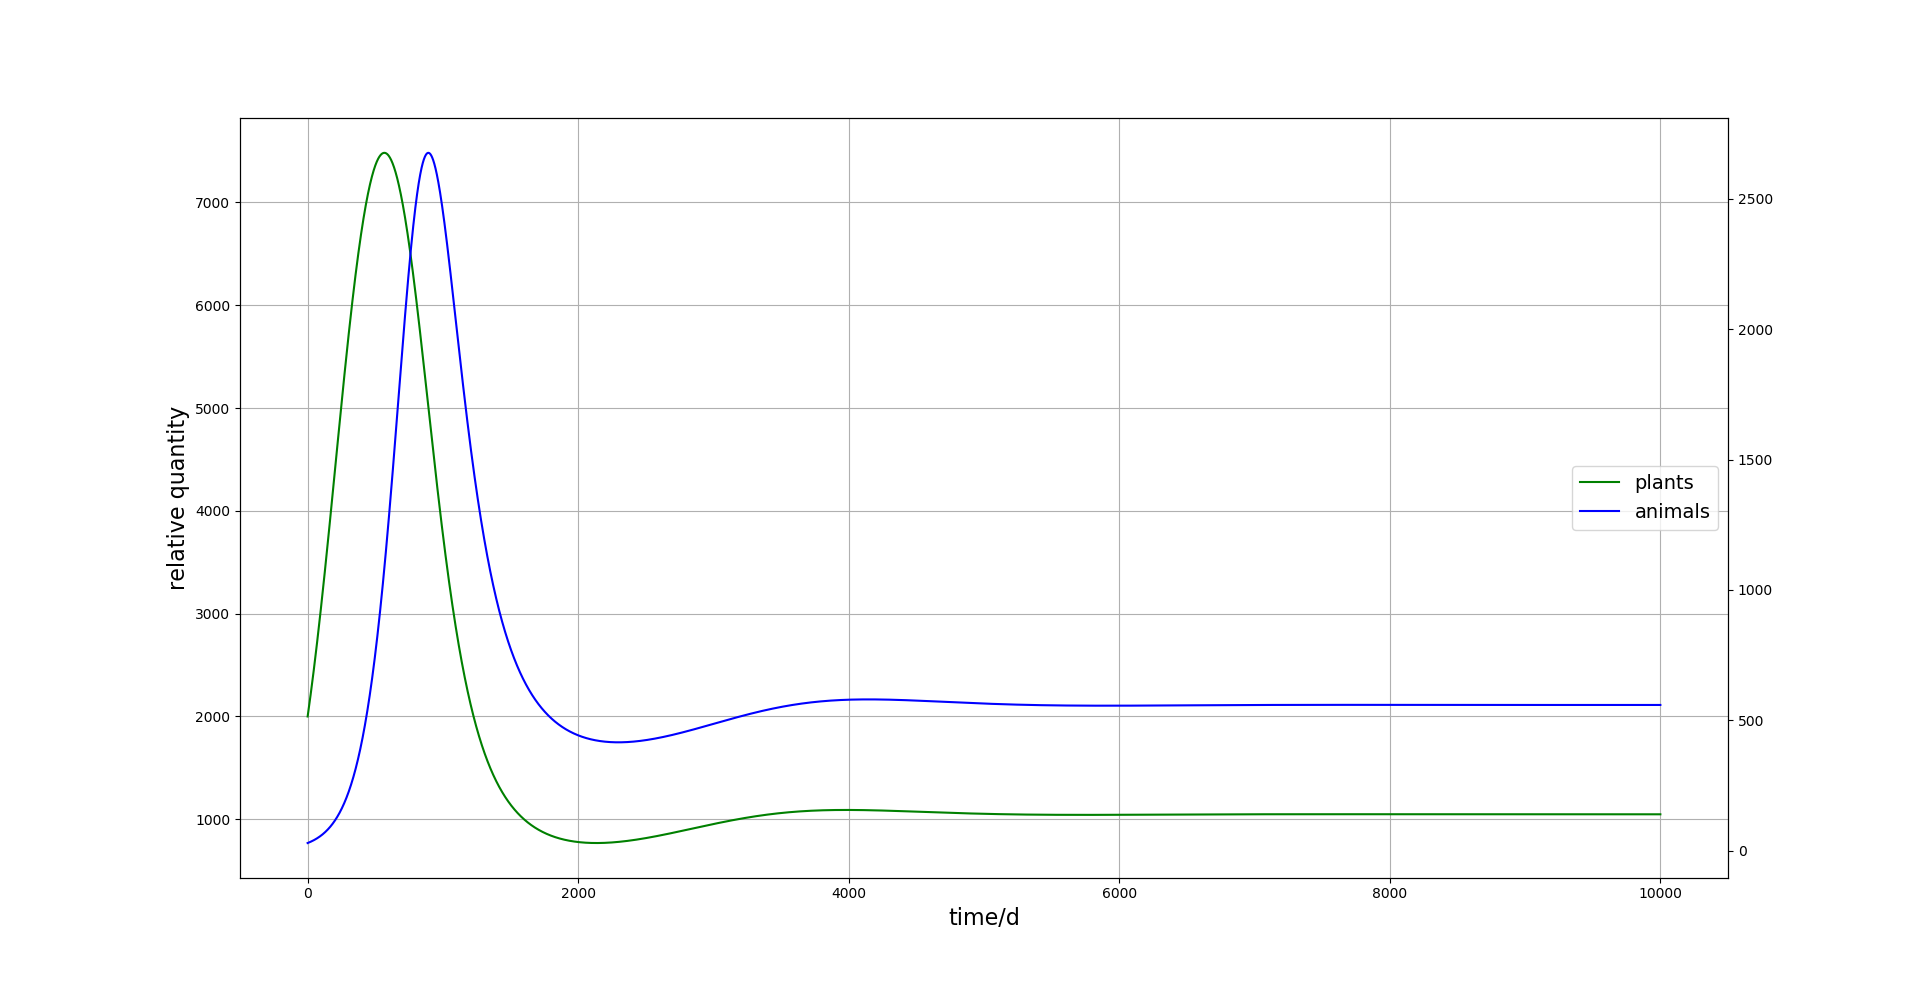
\includegraphics[width=35em]{Figure_9.png}
    \caption{deserts}\label{fig:simulate8}
\end{figure}

Then we put the dragons "using the same survival strategy" into these environments for simulation. The results are shown in the figure, and we can get a conclusion that is consistent with our subjective impression.

In tropical rainforest areas, richer light conditions and rain determine that the natural environment has more capacity and resilience. There are more animals and plants than grasslands. In the face of dragons, such an "invader", the original environment and the dragon reached a balance faster, and were relatively less affected; for the dragon, it seemed to be a good habitat choice.

Dragons who have just migrated to the desert or ice fields are not so lucky. The local natural environment determines that once they arrive in the environment, they will suffer from hunger and leave after a few days of starvation. At the same time, it is also a big blow to the ecosystem: although it is not enough to pay for the huge amount of food for the dragon, the animals within the dragon's range of activity will still be eaten every day, and it will take a certain time to restore to the original state.

Of course, it is not difficult for us to find that because dragons are carnivorous animals who do not care about plants, and even help plants survive and multiply indirectly through carnivorous eating, making it almost impossible for the ecosystem to collapse due to dragons’ massive feeding. As the cornerstone of the ecosystem, plants have the ability to control the restoration of the ecosystem and provide the original energy source for the organisms in the environment as much as possible. In fact, we can see from the previous simulation curve that even if the initial number of animals is almost zero, even if the number of animals leads to a further decline in the number of plants, as long as part of it is preserved, it can help the ecosystem gradually approach balance.




~\ \
\section{Strengths and weaknesses}
~\ \

\subsection{strengths}
~\ \

The model we built can simulate and fit the dragon's growth process, the succession process of the natural environment, and the interaction between the dragon and the natural environment. And through multiple experiments on the same process, the stability of the model is proved; when the model is transferred to a large carnivore that exists in reality, the error between the calculated result and the information shown in the existing literature is acceptable.

Our model takes into consideration the predator’s dynamic strategy and other biological activity laws that are in line with practical significance, making the dragon’s activities more representative and authentic. The amount of resources in nature is quantified by us using appropriate models to improve accuracy.

Although the dragon is a fictitious creature, the results we get can be used in other activities, such as the protection of large wild animals and the maintenance and development of ecosystems. The model has more far-reaching significance.

~\ \
\subsection{weaknesses}
~\ \

Our abstraction of the components of the ecosystem may be oversimplified, so as to ignore the influence of some more complex elements on the interaction between organisms and the system. In addition, the life activities of dragons are simply divided into hunting and growing, and some important things such as reproduction are not taken into consideration.

At the same time, we have also noticed that adopting a certain ratio to directly convert solar radiation into the energy input of the ecosystem is an inaccurate method, which may be an important reason for the error between the result and the actual.

~\ \
\section{Sensitivity Analysis}
~\ \

In the above discussion, we always initialize the ecosystem with an idealized condition, that is, dragons always join the original ecosystem when it reaches equilibrium. So in other cases, how will the dragon interact with the ecosystem? Here we have taken two extreme cases. Figures 11 and 12 respectively show the following situations: 
\begin{enumerate}
\item The number of animals is far less than the environmental capacity; 
\item The number of animals far exceeds the environmental capacity.
\end{enumerate}

\begin{figure}[h]
    \centering
    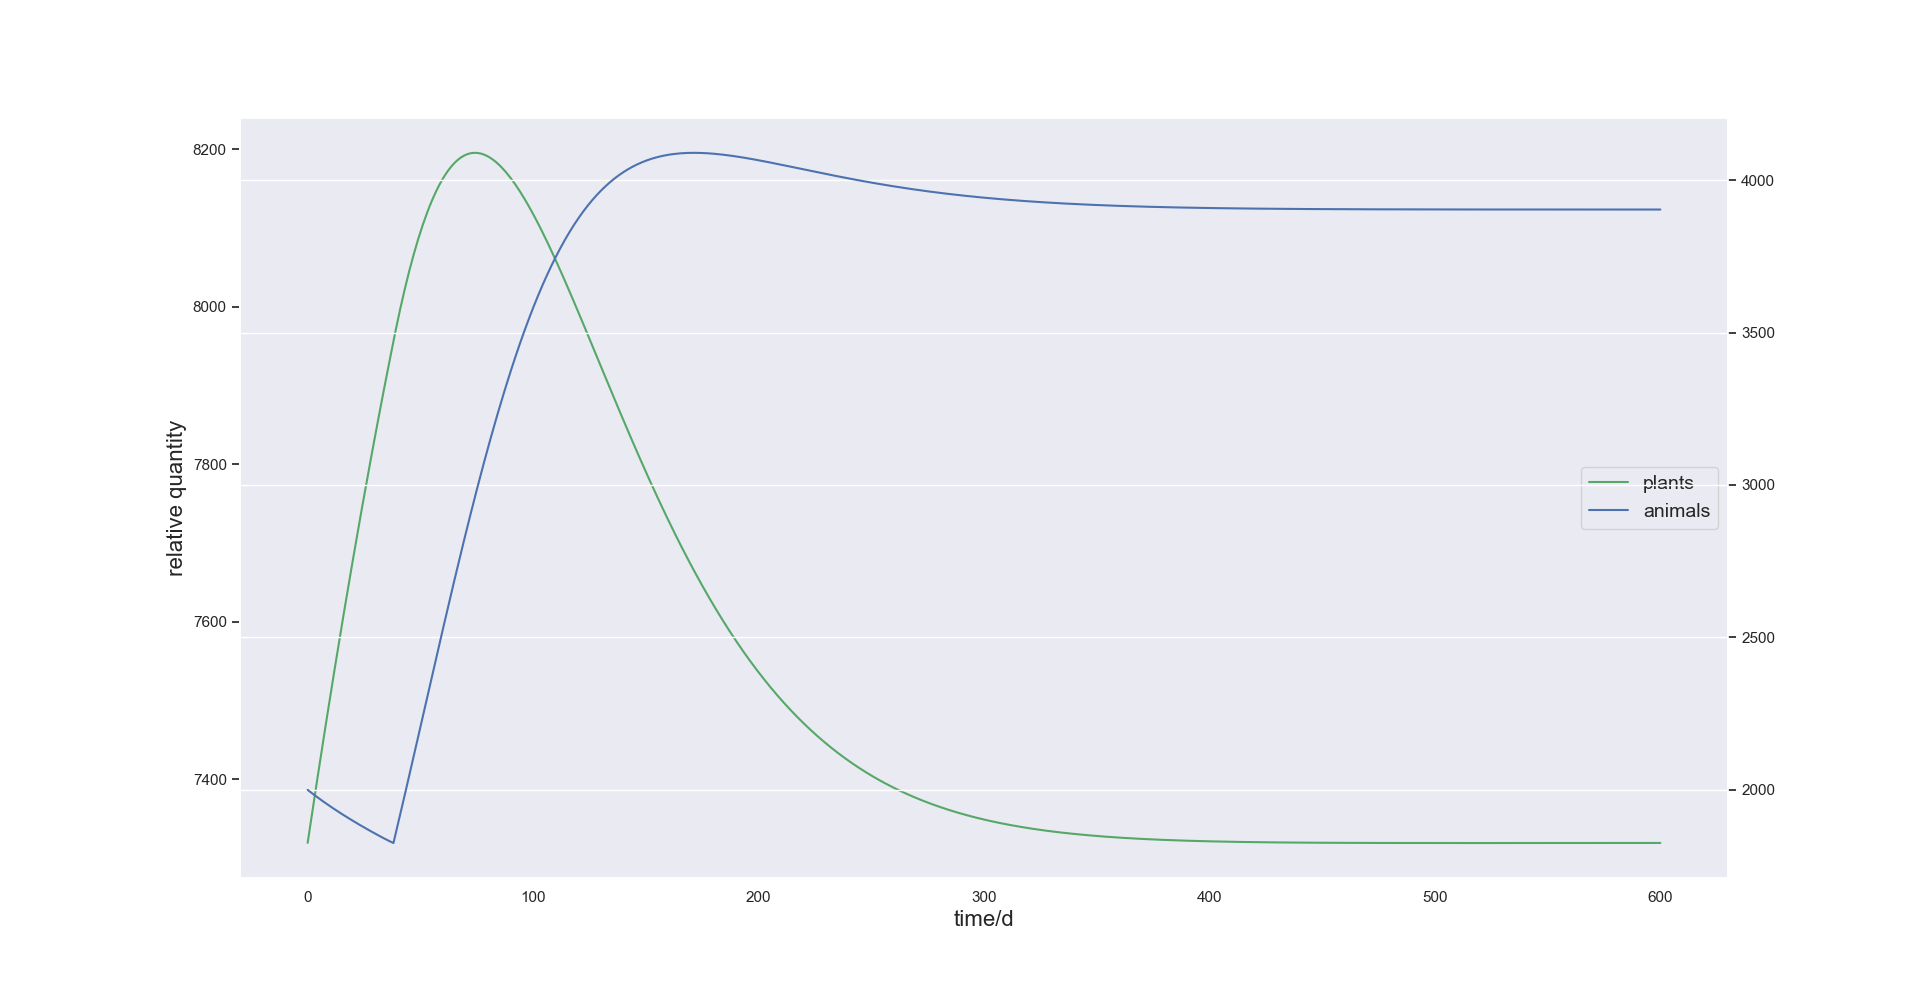
\includegraphics[width=35em]{Figure_11.png}
    \caption{Few animals}\label{fig:simulate9}
\end{figure}

\begin{figure}[h]
    \centering
    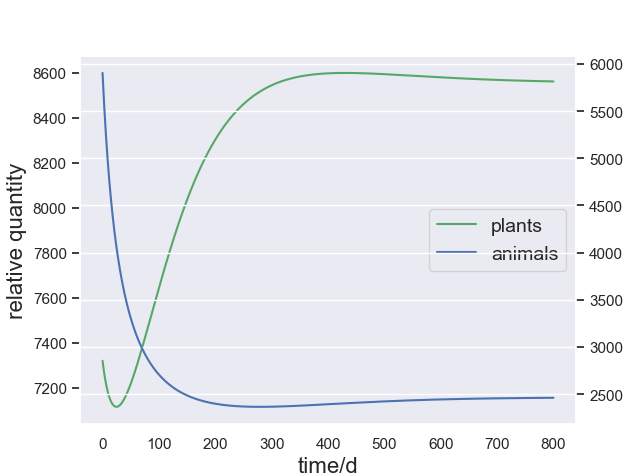
\includegraphics[width=30em]{Figure_12.png}
    \caption{Too many animals}\label{fig:simulate10}
\end{figure}

It is not difficult to see that in the first situation, the dragon left very early due to lack of food, and what is left is the succession effect of general animals and plants. The curve is similar to the situation that happened when the balance was originally carried out; and in the second case, it is almost for the final The state has no effect, but in the early stage, due to insufficient food (plants), the number of general animals will decline rapidly.

From this we can know that when a dragon joins an ecosystem, the situation of the ecosystem is actually affected to a certain extent. Generally speaking, the number of animals in an ecosystem will not exceed the capacity of the environment. Therefore, considering the practical significance, if the dragon chooses to join when it happens to be an animal in an ecosystem, it may miss a potential opportunity to provide a long-term stable living environment due to the current lack of food. 



\newpage
% 以下为信件部分,不需要可自行去掉
% 如有需要可将整个 letter 环境移动到文章开头或中间
\begin{letter}{Letter}
\begin{flushleft}  % 左对齐环境,无首行缩进
\textbf{To:} George R.R. Martin\\
\textbf{From:} Team 1234\\
\textbf{Date:} January 23rd, 2021\\
\textbf{Subject:} 
\end{flushleft}

Dear Mr. Martin:\\

Our team like your book \emph{A Song of Ice and Fire} very much. We have recently considered Daenerys' three dragons seriously. 
We want to know if they can live in the wild alone and what will they bring to the ecosystem. We use some of characteristics
you wrote in the book and make some reasonable assumptions to build models. Our models calculate the growth of the dragons
and simulate their survival in the real world. We'd like to use our models to give some recommendations to you to create
more scientific assumptions about dragons’ characteristics in your book.

We analyse the growth curve to pridict the growth process of dragon, and calculate the energy intake and expenditure of the dragon.Theoretically, the growth curve of dragon is similar to S-shape or sigmoid. They will grow continuously if enough food are provided. Dragons will grow rapidly in the middle time of their life. We calculate that a dragon can grow to nearly 200 tons after four hundred years old. And of course they need huge energy intake to grow when they are already heavy. However, it should be noted that the energy consumed by a dragon to grow to such a size is very huge. For example, a 100-ton dragon needs $2.254 \cdot 10^{10}$ J of energy to gain another one kilogram, and the energy consumed by him every day also reaches an amazing $3.83549 \cdot 10^{8}$ kJ. Therefore it's important to pay attention to match the weight of the dragon and food.

In fact, it is very difficult to raise a dragon. We found that at least 15000 square kilometers of land is needed in the temperate grassland ecosystem to meet the daily energy consumption of a 100 ton dragon. While for a dragon weighing less than 10 tons, it only needs 80 square kilometers of land to meet its energy needs. Considering that Daenerys Targaryen has fed three dragons, you must be very careful to control the weight of the dragons. It's better not to let them exceed 30 tons, otherwise it's almost impossible for the Mother of Dragons to feed them.

If your dragon weighs more than 20 tons, never put it in arid or Arctic regions! We found that for a 50 ton dragon, in temperate grassland areas or other areas more suitable for survival, such as tropical rainforests, the dragon can always reach a balance with the local ecological environment after a period of time; while in arid or Arctic areas, due to the limited energy provided by the environment, the dragon will not get enough food for a long time in less than two months And leave.
Therefore, if you want the dragon to grow stronger, put it in a more suitable environment for animals!

Thanks for your reading our letter. We are your avid reader and we sincerly wish our advice can help you. We welcome your reply
and inquiries about our models.\\

\rightline{Yours sincerely}
\rightline{Team 1234}
\end{letter}

\newpage
% 参考文献

\begin{thebibliography}{99}
\bibitem{1} Nagy, K. "Food requirements of wild animals: Predictive equations for free-living mammals, reptiles, and birds." (2018).
\bibitem{2} Stass, V. L. "An Analytical Model of Animal Growth." European Scientific Journal 13.27 (2017): 1-17.
\bibitem{3} Hairston Jr, Nelson G., and Nelson G. Hairston Sr. "Cause-effect relationships in energy flow, trophic structure, and interspecific interactions." The American Naturalist 142.3 (1993): 379-411.
\bibitem{4} Beschta, Robert L., and William J. Ripple. "Large predators and trophic cascades in terrestrial ecosystems of the western United States." Biological conservation 142.11 (2009): 2401-2414.
\bibitem{5} Ripple, William J., and Robert L. Beschta. "Large predators limit herbivore densities in northern forest ecosystems." European Journal of Wildlife Research 58.4 (2012): 733-742.
\bibitem{6} Schoener, Thomas W. "Models of optimal size for solitary predators." The American Naturalist 103.931 (1969): 277-313.
\bibitem{7} Tschirhart, John. "A new adaptive system approach to predator–prey modeling." Ecological Modelling 176.3-4 (2004): 255-276.
\bibitem{8} Penguin Random House (2018). A Song of Ice and Fire Series. Retrieved from https://www.penguinrandomhouse.com/series/SOO/a-song-of-ice-and-fire/.
\end{thebibliography}

\newpage
% 以下为附录内容
\begin{appendices}
\section{program source code}
Here are python programmes we used in our model to calculate pairwise comparison matrix as follow.\\
\textbf{\textcolor[rgb]{0.98,0.00,0.00}{python program source:}}
\lstinputlisting[language=python]{./code/GragonEcoSimulation.py}

\end{appendices}
\end{document}


